\section{Průzkum požadavků škol}
\change{rephrase}
Tvorba začala zjištěním požadavků. Udělal jsem Google formulář, který primárně zjišťoval informace o školním systému. Pomocí vedení školy byl pak rozeslán na spřátelené střední školy. 
\subsection{Výsledky průzkumu informačních systémů středních škol}
Na dotazník odpovědělo 13 škol z moravskoslezského kraje.

\begin{figure}[h]
    \centering
    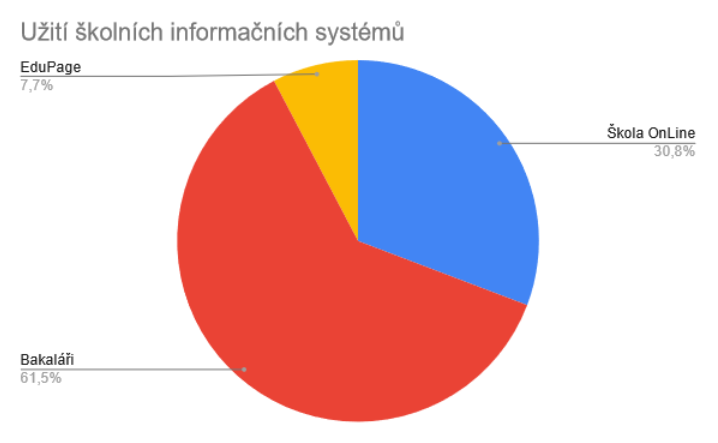
\includegraphics[width=0.5\linewidth]{Figures/vyuziti_skolnich_systemu.PNG}
    \caption{Využití školních informačních systémů}
    \label{fig:vyuziti-skolnich-systemu}
\end{figure}

Většina škol používá systém Bakaláři a na něj se bude zaměřovat import. Import bude možné udělat z tiskových sestav. Pro jiné školní systémy bude možno použít XML import, který je univerzální (podporuje i Bakaláře\footnote{Je však potřeba přístup k databázi Bakalářů a speciální program na vygenerování XML.}).


\newpage

\begin{figure}[t]
    \centering
    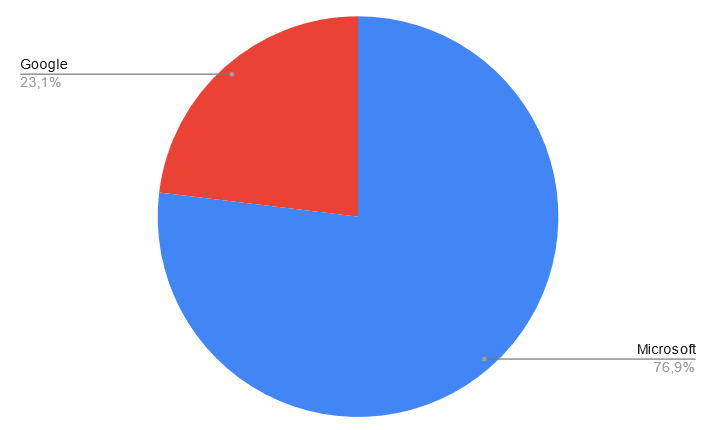
\includegraphics[width=0.5\linewidth]{Figures/poskytovatele_emailu.PNG}
    \caption{Poskytovatelé emailů}
    \label{fig:poskytovatele-emailu}
\end{figure}

Všechny dotazované školy mají emaily od Microsoftu nebo Googlu.
Přihlašování bude probíhat pomocí emailu. Uživatelé se budou moci přihlásit do portálu pomocí protokolu OAuth, který podporují oba provozovatelé. Výhodou tohoto způsobu přihlašování je, že naše aplikace neukládá hesla. Alternativně je možné ukládat heslo\footnote{Zahashované funkcí Bcrypt} do lokální databáze.



\section{Návrh databáze}

Při návrhu databáze jsme počítali, že aplikace bude jen pro jednu školu (single tenant), prakticky to znamená, že nebude entita škola. 
Podpora nasazení pro více škol je řešena pomocí konteinerizace.
Entity, které jsou importovány jsou úzce modelované podle zdrojů importu.

Rozhodli jsme se, že \codename{EvaluationUnit}\footnote{Jedná se o úvazek, který je hodnocen. Je spojením učitele, skupiny, předmětu. Někdy v kódu importu nazýván \codename{TaughtSubject}.} 
nebude mít M:N vztah se skupinami, to zjednodušuje celou aplikaci, až na import kde je potřeba spojovat více skupin do jedné skupiny.
Existuje však \codename{MultiClassGroup}, což je skupina složená z více skupin, ta je však pouze použita v kroku spojování skupin (\ref{postup:spojovani-skupin}).
Tato entita je nutná, aby bylo možné opustit import a později se k němu vrátit.

Údaje o importech se nachází v \codename{ImportStatus}. Ten má relace na všechny \codename{ImportedEntity}, aby byl znám původ instance dané entity.

Přikládám ER diagram (\improvement{pridat er diagram ref}). Jedná se pouze o schéma databáze, jak ho Doctrine namapovala.

Nejde v něm vidět dědičnost u uživatelů, dědičnost je mapována strategií Class Table Inharitance\cite{P-of-EAA}.



\improvement{Vložit schéma db: }



\section{Způsoby importu}
Při prvotním importu, kdy se načítají informace o studentech a úvazcích se rovnou vytváří entity. Entity se ale nepersistují hned a ukládají se do databáze až v ImportService.

Importy z XML a sestav splňují interface \codename{ImportDataProvider}. Ten se skládá z getterů vracejících managery. Managery jsou objekty, co se starají o správu daných entit. \codename{ImportService} potom příjme \codename{ImportDataProvider} a postará se o jeho uložení. \codename{ImportService} se dá doplnit o další postup ukládání typu \codename{ImportSaveStep}, další postup závisí na formátu ze kterého se importuje.

\section{Import z tiskových sestav systému Bakaláři}
\improvement{proofread}
Tento typ importu slouží pro školy, které nemají přístup k databázi Bakalářů. 
Jedná se primárně o školy, které využívají cloud verzi Bakalářů. Využívají se tři sestavy, které jsou již předvytvořené\unsure{Doufám, že nejsou custom}. Bakaláři používají XFRX\footnote{Knihovna, která převádí Visual FoxPro reporty na elektronické sestavy různých formátů} ke generování samotných sestav. Tyto sestavy nejsou určeny ke zpětnému programatickému čtení dat.

Dostupné formáty sestav jsou TXT, CSV, XLS a HTML. U sestav formátu TXT chybí mezery jako separátor u sloupců, sestava předmětů ve formátu CSV by byla možná importovat, ale ostatní sestavy by nešly jednoduše zpracovat kvůli zdánlivě náhodnému počtu separátorů, podobný problém nastává i u XLS tam se však ještě vyskytuje problém se sloučenými poli.

Zvolil jsem, že budu importovat HTML sestavy. Celá tabulka je postavená na základě absolutního pozicování. Při parsování sestav seřadím jednotlivé divy podle absolutního pozicování. Tímto způsobem převádím každý řádek v tabulce na objekt.

Sestava úvazků však obsahuje řadu chyb. Když učitel zárověň učí více tříd najednou, objeví se ve sloupci třídy nevalidní zkratky tříd. Toto řeším vyhledáním třídy a skupiny v sestavě tříd na základě členů skupiny. 
Zkratky předmětu jsou správné, až na případ když se daný předmět dělí na teorii a cvičení,
kvůli tohoto je potřeba najít v sestavě předmětů správnou zkratku. Někdy se stane, že název předmětu není úplný a potom se vezme zkratka ze sestavy předmětů.

Nula ve sloupci týdně znamená, že daný učitel tento úvazek\unsure{co je uvazek} aktuálně neučí, to muže nastat při rotaci skupin nebo u teorií daného předmětu, které učitel neučí\improvement{rephrase}. 

\begin{figure}[h]
    \centering
    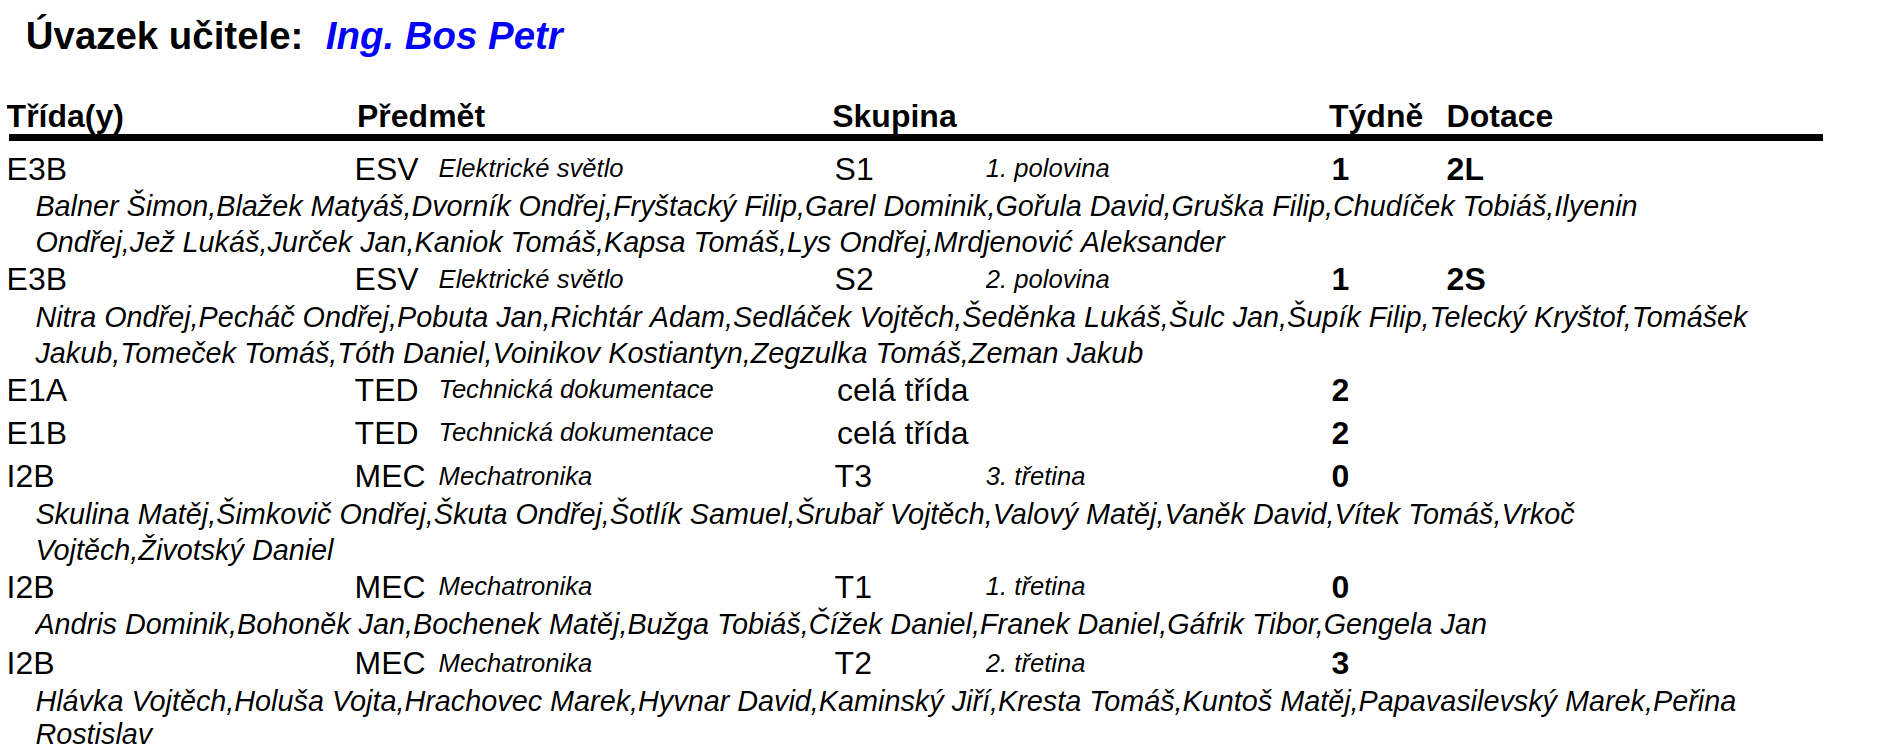
\includegraphics[width=1\linewidth]{Figures/uvazky-ucitelu-ukazka.png}
    \caption{Ukázka sestavy obsahující úvazky učitelů}
    \label{fig:uvazky-ucitelu-ukazka}
\end{figure}

\begin{figure}[H]
    \centering
    
\includegraphics[width=1\linewidth]{Figures/skupiny-ukazka.png}
    \caption{Ukázka sestavy rozdělení studentů do tříd}
    \label{fig:ukazka-sestavy-tridy}

\end{figure}
\begin{figure}[H]

    \centering
    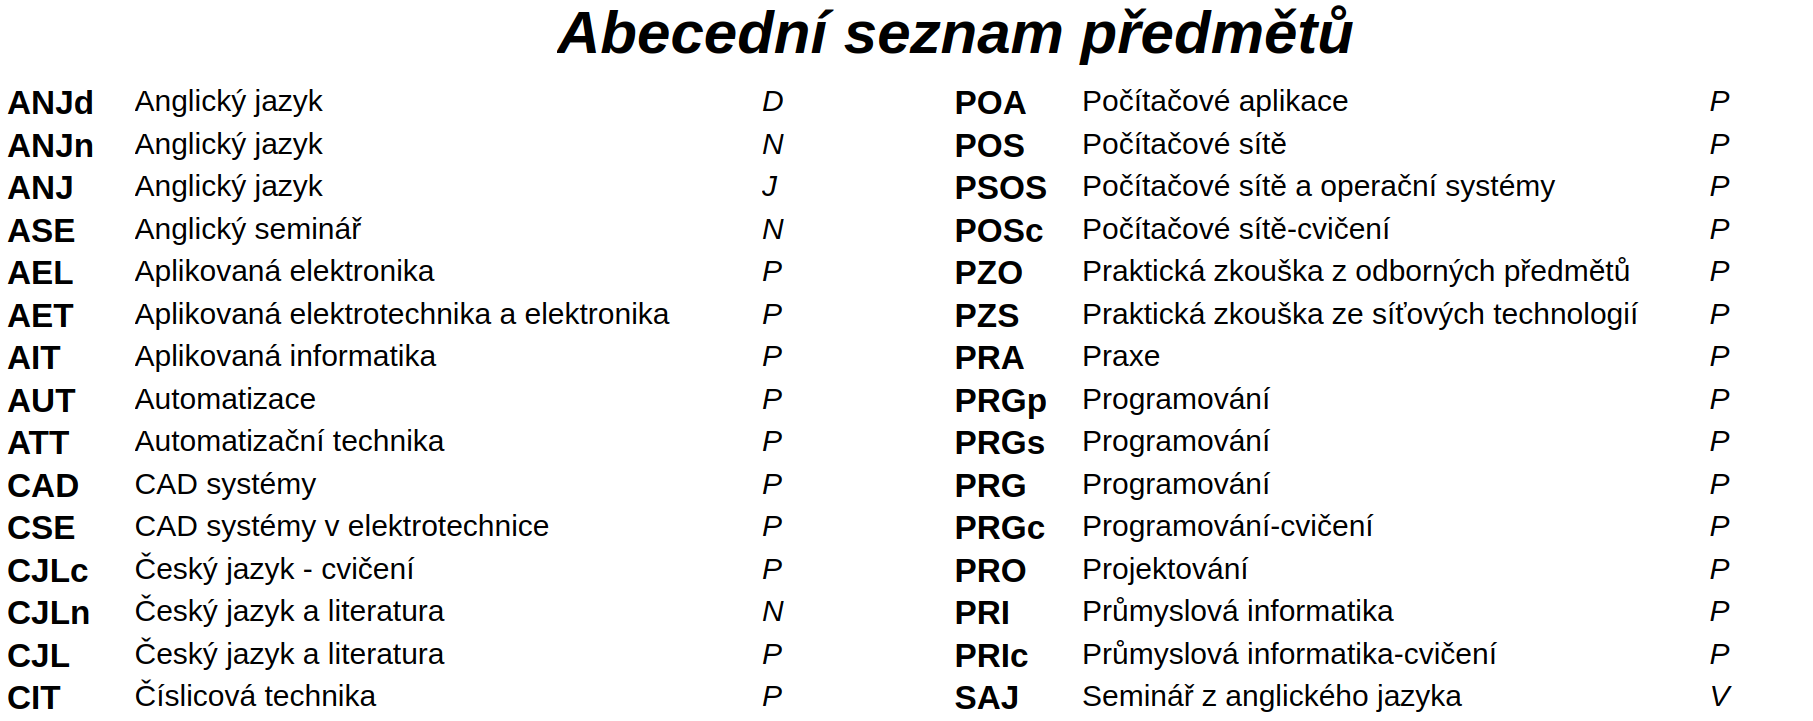
\includegraphics[width=1\linewidth]{Figures/predmety-ukazka.png}
    \caption{Ukázka sestavy předměty}
    \label{fig:ukazka-sestavy-predmety}
    
\end{figure}

\begin{code}[H]
  \begin{minted}[breaklines]{html}
<div class="page" style="width:794;height:1123;"><a name="XFRXPAGE_1">
 ...
 <div class="font7" style="top:30px;left:129px;...">Ing. Bos Petr</div>
 <div class="font6" style="top:30px;left:4px;...">Úvazek učitele:</div>
 <div class="font2" style="top:103px;left:8px;height:30px;width:745px;...">Balner Šimon,Blažek Matyáš,Dvorník Ondřej,Fryštacký Filip,Garel Dominik,Gořula David,Gruška Filip,Chudíček Tobiáš,Ilyenin</div>
 ...
</div>
\end{minted}
\caption{Zkrácené zdrojový kód HTML sestavy úvazky učitele}
\end{code}


\section{Import z XML}
Import z XML je nezávislý na školním systému. Je však potřeba mít externí program, který XML vytvoří dle daného RelaxNG schématu (schéma je v souboru \codename{Bakalari.rng}). Struktura je použitá z předchozí verze (více v \ref{uvod:predchozi-verze}), kořenový prvek se jmenuje \codename{BakalariImport} z historických důvodu. Emaily jsou v dobrovolné a pokud budou u některých studentů/učitelů chybět vygenerují se v dalším kroku importu.

Na import XML se používá PHP extension SimpleXML. Je to jednoduchý způsob parsování. Jediná nevýhoda je, že SimpleXML načte celý soubor XML do paměti. XML soubory škol jsou však malé a i kdyby měla škola počet žáků v řádech tisíců, SimpleXML by dostačovalo. 



\definecolor{gray}{rgb}{0.4,0.4,0.4}
\definecolor{darkblue}{rgb}{0.0,0.0,0.6}
\definecolor{cyan}{rgb}{0.0,0.6,0.6}

\begin{code}[H]
  \begin{minted}[fontsize=\small]{xml}
<?xml version="1.0" encoding="utf-8"?>
<BakalariImport>
    <SkolniRok>2022/23</SkolniRok>
    <Predmety><Predmet><Zkratka>PRG</Zkratka>
    <Nazev>Programování</Nazev></Predmet>
    </Predmety>
    <Studenti>
        <Student>
            <Jmeno>Marek</Jmeno>
            <Prijmeni>Konrád</Prijmeni>
            <!-- Email není povinný -->
            <Email>m.konrad.st@spseiostrava.cz</Email>
            <Trida>I4C</Trida>
            <Skupiny><Skupina>S1</Skupina></Skupiny>
        </Student>
    </Studenti>
    <Ucitele>
        <Ucitel>
            <Jmeno>Vlasta</Jmeno>
            <Prijmeni>Kubinová</Prijmeni>
            <Titul>Mgr.</Titul>
            <!-- Email není povinný -->
            <Email>v.kubinová@spseiostrava.cz</Email>
            <Zkratka>NOW</Zkratka>
            <Predmety>
                <Predmet>
                    <Zkratka>PRG</Zkratka>
                    <Tridy>
                        <Trida>
                            <Zkratka>I4C</Zkratka>
                            <Skupina>S1</Skupina>
                        </Trida>
                    </Tridy>
                </Predmet>
            </Predmety>
        </Ucitel>       
    </Ucitele>
</BakalariImport>
\end{minted}
\caption{Ukázka struktury XML}
\end{code}


\section{Databáze a mapování importu}

Importy závisí na školní rok. Když vytvoříte školní rok nemáte žádná data. Každé hodnocení probíhá od začátku školního roku až po moment nejnovějšího importu.

Ukládání importu do databáze probíhá pomocí ORM. Máme vytvořené třídy a Doctrine už je mapuje na tabulky v relační databázi. Doctrine dokáže mapovat celou řadu OOP konceptů jako dědičnost a kompozici.

Uživatele máme řešené dědičností tak, že třídy \codename{Student} a \codename{Teacher} dědí z abstraktní třídy \codename{ImportedPerson} a ta dědí ze třídy \codename{User}. Takto uspořádaná hierarchie tříd má řadu výhod jako možnost dotazovat všechny importované osoby najednou.   Toto se používá v řešení duplikátu emailu (\ref{postup:deduplikace-emailu}).\improvement{toto se využívá v ... ref} Nevýhoda takovéhoto mapování je zvýšená komplexita pro ORM a potencionální degradace výkonu z databázové strany.

Doctrine je ORM se silnou abstrakcí, což značně komplikuje samotné ukládání. Není totiž podporovaná operace \textsc{upsert} (v databázi PostgreSQL realizovanou pomocí jednoho dotazu \textsc{insert into ... on conflict do update}). Je sice možné užít nativní SQL, ale tím bychom přišli o výhody ORM.
Nevýhodou je pomalejší ukládání, to se děje kvůli tomu, že Doctrine se snaží vytvořit graf daných entit, Doctrine interně používá identity map na entity takže je vyšší spotřeba RAM.



\section{Inkrementální import}

Zdroje importů nemusí poskytovat data o celém školním roce, v případě importu ze sestav se jedná o úvazky, kde se střídají skupiny u učitele (na naší škole např. mechatronika).
 Nebo se během školního roku něco nečekaně změní.

Proto umožňujeme inkrementální import, importuje se jen to nové a staré importy nechává nedotčené. Doporučuji dělat import před každým testovacím obdobím. Data ze starých importů není třeba odstraňovat (i staré úvazky, které už nemusí být platné lze hodnotit). 

Entity spravované importem implementují interface \codename{ImportedEntity}.

\begin{code}[H]
\begin{minted}{php}
  <?php
    interface ImportedEntity
    {
        public function getId(): mixed;
        public function getImportHash(): ?string;   
        public function loadImportHash(): string;   
        public function updateFromSelf(ImportedEntity $old): static;
    }
\end{minted}
\caption{Zdrojový kód \codename{ImportedEntity}}
\end{code}

V Doctrine se dělají hromadné operace po $N$ operacích. $N$ se dá zvolit experimentem.
Po každých $N$ operacích se pak zavolají metody \codename{EntityManager.flush()} a \codename{EntityManager.clear()}. Dělá se to po inkrementech, aby \codename{UnitOfWork} byl schopen udělat možné optimalizace a aby se zamezilo zbytečnému procházení grafu entit. Operace clear pak vyčistí graf, to je důležité aby nedošlo k úniku paměti.

\codename{ImportedEntity} má metody loadImportHash ta se používá ke vytvoření import hashe. Import hash se skládá z atributů, které unikátně identifikují danou entitu. Pro import nelze spoléhat na dané atributy, protože uživatel je může prostřednictvím administrace upravit. To by znamenalo, že při dalším importu bude stejná instance entity znovu vytvořena\footnote{Kdyby chtěl uživatel, aby byla při dalším importu vytvořena nová instance entity, může vymazat hodnotu import hashe.}.
Import hash je využíván třídou \codename{ImportedEntityUpsertProcessor}. Ten se stará o upsert importovaných entit.
\codename{ImportedEntityUpsertProcessor} načte při upsertu všechny instance ukládané entity.
Potom vytvoří \codename{entityMap}, což je mapa import hashů na id.
Pak se prochází instance entit, které byly právě naimportovány a pokud nejsou v \codename{entityMap} tak se uloží pomocí hromadné operace a staré \codename{ImportedEntity} se upraví pomocí metody \codename{updateFromSelf}\footnote{Tato operace nemusí být využita}.


\section{O korcích importu}

Kroky importu jsou nezávislé na zdroji importu. 
Jedná se o import wizard, kdy konečný automat \vizref{uvod:konecny-automat} rozhoduje o dalším možném stavu. 
Na obrázku \ref{postup:import-diagram} je diagram korků importu.
\improvement{Diagram workflow}


U definice tohoto konečného automatu je v metadatech stavu uložen presenter, který má za úkol zobrazení a zpracování daného stavu.
Presenter je vlastně interface. Presentery jednotlivých kroků jsou buď přímo implementují interface nebo dědí z abstraktních tříd
pro jednotlivé použité frontendové technologie (\codename{LiveComponentPresenter}, \codename{FormPresenter}\unsure{fact check names}).

Tím, že presenter vrací pohled je možné, aby krok importu vypadal jakkoliv.
K importu bylo využito hodně knihoven ze Symfony UX.
Používám Symfony Form na formulář pro zadání souborů a generování emailu.
Na spojování skupin používám LiveComponent, takže celý import obsahuje jen minimum JavaScriptu.

Zpracování jednotlivých kroků může trvat dlouho, a proto používám na přechody mezi kroky Hotwire Turbo \vizref{ux-turbo}.
Celý krok je v HTML elementu \codename{turbo-frame\unsure{turbo element name ?}}, ten je při odeslání formu nahrazen novým framem\footnote{Není úplně nahrazen, ale je pomocí DOM morph knihovny upraven}. 


\clearpage

\begin{sidewaysfigure}
	\centering
  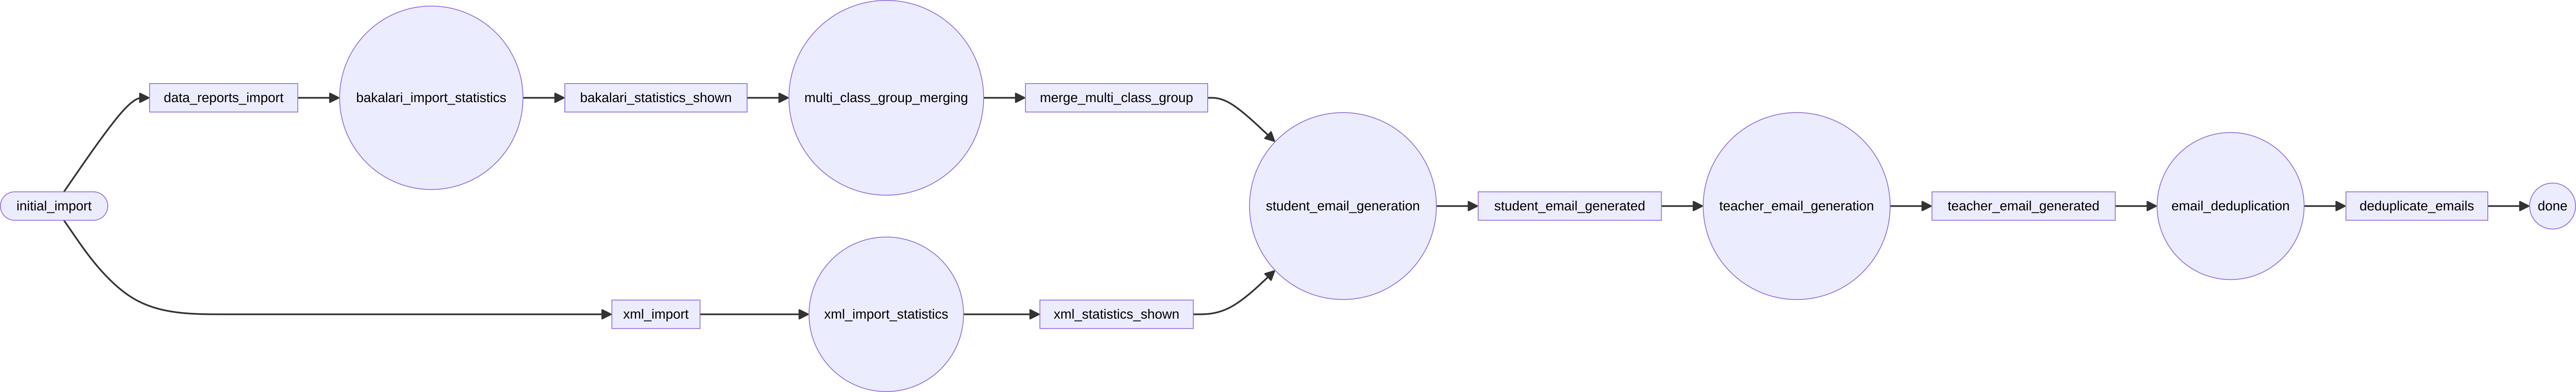
\includegraphics[width=1\linewidth]{Figures/import-diagram.png}
  \caption{Diagram konečného automatu pro koky importu}
  \label{postup:import-diagram}
\end{sidewaysfigure}

\clearpage

\section{Generování emailů z uživatelských dat}

Tím, že zdroje importu nemusí nutně poskytovat email, umožňuji generování emailu.
Emaily se generují jak studentské, tak učitelské.

Emaily se generují pomocí speciálních výrazů.
Výrazy jsem vymýšlel tak, aby byly pro uživatele co nejjednodušší.
Skládají se z řetězcových proměnných a konstant, hodnoty proměnných a konstant se potom spojí do jednoho výsledného řetězce, který je potom validován zda se jedná o email. V případě, že řetězec není validní email nastaví se u daného uživatele tag vyžaduje úpravu. 

Proměnné jsou ve výrazu ohraničeny \textit{()}. Závorky můžou být validní v emailu pokud je lokální část emailu ohraničena uvozovkami\cite{wiki-email-address}. To by však neměl být problém, jelikož RFC5321 specifikuje, že emailové schránky, které se využívají k posílání emailů by neměly mít lokální část ohraničenou uvozovkami\cite{rfc5321}.

Proměnná se dá vložit celá \textit{(jmeno)}, znak \textit{(jmeno[1])} nebo rozsah znaků \textit{(jmeno[1:3])}.
Ukázkový výraz pro studenty naší školy by tedy mohl vypadat takto \textit{(jmeno[1]).(prijmeni).st@spseiostrava.cz}.

Tento krok importu je realizován pomocí Symfony Form. Zajímavý je vstup do kterého se zadává emailový výraz. Jedná se o samotný formulářový typ, ty se dají do sebe vnořovat a výsledný formulář má taktéž typ formuláře. 

To pole využívá editor Ace, který je velice přizpůsobitelný, ať už vzhledově nebo funkčně. Rozšířil jsem Ace, aby se choval jako formulářový prvek a přidal jsem zvýrazňování emailových výrazů.

\section{Úprava duplicitních emailů}\label{postup:deduplikace-emailu}

Při generování výrazů může nastat duplicita emailů.
Na naší škole se musí duplicita řešit u zhruba 2\% studentů.
Duplikátů je malý počet a jejich řešení se řeší manuálně.
Při řešení změně emailů může dojít k jiné kolizi emailů to se řeší tak, že tento krok probíhá dokud existují duplikátní emaily. Kolize muže nastat mezi emaily jakýchkoliv importovaných uživatelů, prakticky to znamená, že může nastat kolize studentského a učitelského emailu.

Tento problém mi z velké části pomáhá řešit Doctrine mapováním dědičnosti.
Neprovádí se dotaz s entitou \codename{Student} nebo \codename{Teacher}, ale dotazuje se přímo z entitou \codename{ImportedPerson}\footnote{V Doctrine se dotazuje pomocí DQL a dotazuje se objektový model a ne relační schéma.}.
Jedná se o vnořený dotaz.
Vnější dotaz vybere importované osoby, které obsahují email z výsledku vnitřního dotazu (operátor \textsc{IN}).
Ve vnitřním dotazu se vyberou emaily, které nejsou unikátní. V praxi jsem však dotazy musel rozdělit na dva.\unsure{potencial fix ?}

Tento krok je realizován čistě pomocí Symfony Form. Celý formulář se skládá z pole \codename{CollectionType}\unsure{fact check pls} a \codename{SubmitType}.
  Jako typ kolekce je určen typ formuláře pro importované osoby. Takto nastavený Symfony Form jednoduše určí velikost výsledného formuláře na základě počtu prvků v poli. A při zpracování formuláře mi poskytne zvalidované pole importovaných osob.

\section{Spojování skupin}\label{postup:spojovani-skupin}

Tento krok je nutný pouze u importu ze sestav (viz. \ref{postup:import-diagram}).
V sestavách se nachází pouze informace o učiteli, skupině, třídě a předmětu, nenachází se tam informace o spojení skupin.
Může se stát, že třídy jsou spojené tak, že nelze poznat jestli jsou dané skupiny učeny současně.
Např. Nechť máme třídy $A$ a $B$, kde chlapci a děvčata mají rozdělený tělocvik.

\begin{table}[h!]
\centering
\begin{tabular}{ | c | c | c | }
\hline
 \multicolumn{3}{|c|}{\textbf{Úvazek učitele:} Jan Novák}\\
     \hline
 \textbf{Třída(y)} & \textbf{Předmět} & \textbf{Skupina}\\
 \hline
 A, B & TEV & Chl \\ 
 \hline
 A, B & TEV & Chl \\  
 \hline
 A, B & TEV & Dív \\ 
 \hline
 A, B & TEV & Dív \\  
 \hline
\end{tabular}
\caption{Ilustrační tabulka k příkladu.}
\end{table}

Z takového výčtu nelze poznat jak jsou skupiny spojeny.
Proto jsem vytvořil tento krok. 
Seskupování funguje následovně.
První si administrátor zvolí kombinaci \textit{třídy-předmět-učitel}, které přiřadí skupiny. 
Když se jedná o úvazek, který je učen zvlášť zvolí možnost duplikace kombinace \textit{třídy-předmět-učitel}. Administrátor toto opakuje dokud nepřiřadí všechny skupiny.

\section{Zrušení importu}

Během importování může nastat stav, který si uživatel přeje vrátit.
To se může například stát když napíše špatný výraz na generování emailu.
Tohle je řešeno pomocí možnosti zrušit import.
Tato možnost je dostupná i po dokončení importu pro $N$ nejnovějších importů v daném roce.

Pomocí entity \codename{ImportStatus} se uchovávají informace o importech, jak probíhajících, tak dokončených.
Každá importovaná entita má atribut \codename{import} typu \codename{ImportStatus} \improvement{pridat ref}.
A při rušení importu jsou instance entit z daného importu smazány z databáze.
Jestliže se jedná o zrušení $N$ nejnovějších importů tak se před mazáním filtrují importy na základě školního roku, aby nedošlo ke smazání importů z jiného školního roku.

